% set 0 inch indentation
\setlength{\parindent}{0in} 
% set paragraph space = 1 space
\setlength{\parskip}{1em}
% set line space 1.5
\setlength{\baselineskip}{1.6em}

\setlength{\footskip}{8mm}

\chapter{Literature Review} 
\label{ch:literature-review}

\section{Fall}
\label{Fall}
\paragraph{}
Falls happen to people of all ages, but older people have a high probability of being  harmed and are more likely to fall, especially if they have an abnormal health conditions or balance problems. Falls are a common, but often disregarded, cause of injury. As statistic, Around 1 in 3 adults over 65 and half of people over 80 will have at least one fall a year \cite{nhs_2019}. Most falls do not result in serious injury. But there is always a risk that a fall could lead to broken bones, and it can cause the person to have paralysis. In addition, the level of injury depends on time assistance. Unintentional falls can cause severe injuries and even death, especially if no immediate assistance is given.

\subsection{Fall Detection}
\paragraph{}
Let’s start with the trend of fall detection, as illustrated in Figure \ref{fig:fall_trend}, the data is downloaded from Google Trends with the search topic ‘Fall Detection’. It can be observed that the fall detection topic has gotten more attention and significantly increased in 2019. The several researchers selected to use different sensors and methods depending on their proposes and technological industry. Consequently, it can prove that this topic is what people interested in and  becomes more popular in nearly future.


\begin{figure}[H]
  \centering
  \caption[Fall detection trend]{\emph{Interest of “Fall Detection” overtime from 2004 to present.}}\label{fig:fall_trend}
  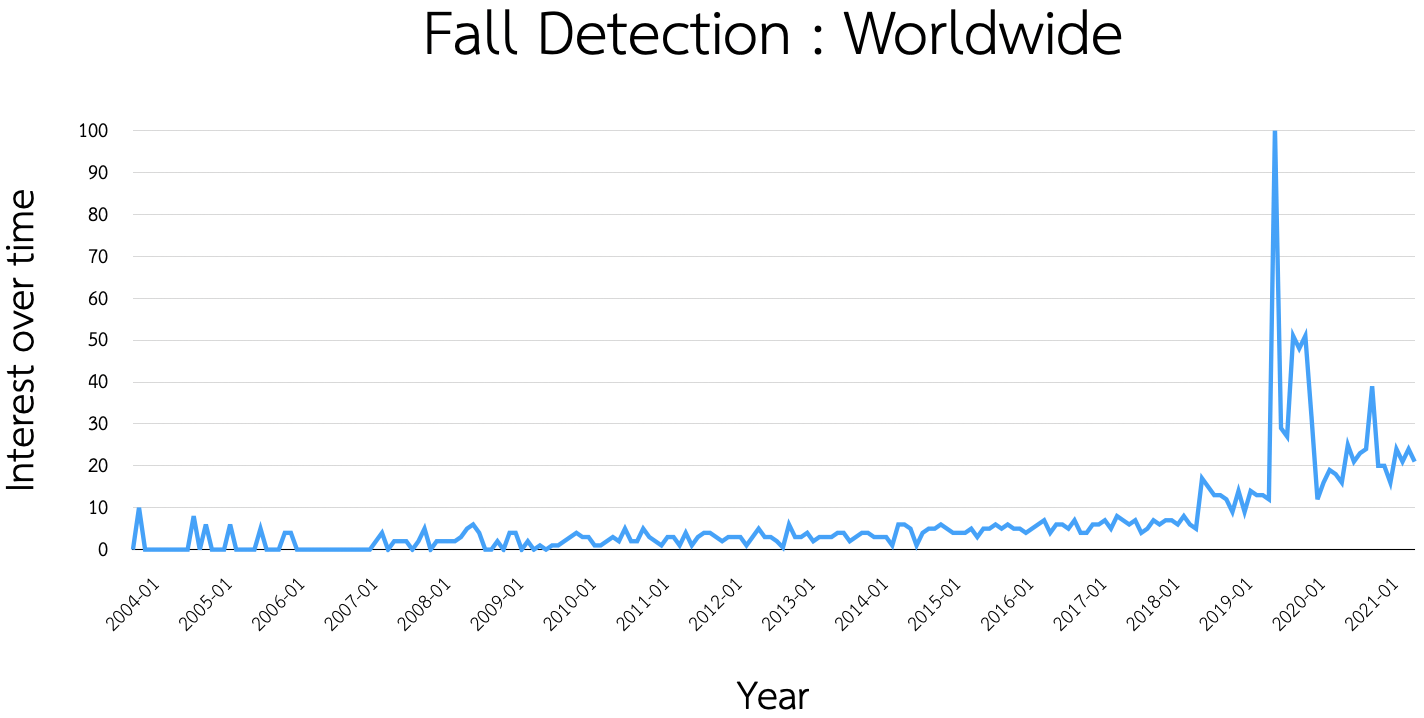
\includegraphics[width=\textwidth]{figures/fall_trend.png}  
\end{figure}

\subsection{Fall Detection by using Vibration sensor}
\paragraph{}
In the Table \ref{tab:fall_review}, it shows the evolution of fall detection from floor vibration. It can be notice that most of them used classifier model to detect the fall event by using simulated fall data which they were not actual fall. Furthermore, they do not deploy their system in the real environment which cannot guarantee an actual performance of model. Thus to overcome these weaknesses, author would like to apply anomaly detection approach to compensate rarely falling down data or unseen pattern, and send alert to caretaker or assistance who always can take care lonely victim as soon as possible.

\begin{table}[H]
\begin{center}
\linespread{0.55}\selectfont\centering
\caption[Summary of literature review for fall detection from floor vibration]{Summary of literature review for fall detection from floor vibration \\}\label{tab:fall_review}
\begin{tabular}{m{0.13\textwidth} m{0.23\textwidth} m{0.20\textwidth} m{0.18\textwidth} m{0.1\textwidth}}
  \textbf{Authors} & \textbf{Data Collection} & \textbf{Related Sensors} & \textbf{Algorithms} & \textbf{Alarm}\\
\hline
\shortciteA{Alwan_2003}& Simulated by people.& N/A&  \begin{itemize} \item Threshold \end{itemize}& N/A \\
\hline
   \shortciteA{alwan_rajendran_kell_mack_dalal_wolfe_felder_2006}& Simulated by people and dummies. & \begin{itemize} \item Piezoelectric \end{itemize} & \begin{itemize} \item Threshold \end{itemize} & Send messages to a pager \\
\hline

\shortciteA{litvak_zigel_gannot_2008}& Simulated by people and dummies.& \begin{itemize} \item Microphone \item Accelerometer  \end{itemize} & \begin{itemize} \item Gaussian model \item Suquential forward floating selection (SFFS)  \end{itemize} & N/A \\
\hline


\shortciteA{davis_caicedo_langevin_hirth_2011} & Simulated by people. & N/A & \begin{itemize} \item Threshold \end{itemize}& N/A \\
\hline

\shortciteA{inproceedings}& N/A & \begin{itemize} \item Pyroelectric infeared (PIR) \item Vibration sensor\end{itemize}& \begin{itemize} \item Support vector machine (SVM) \end{itemize} & N/A\\
\hline


\shortciteA{shao_wang_song_ilyas_guo_chang_2020} & Simulated by 3d-printed skeleton & \begin{itemize} \item Accelerometer\end{itemize} & \begin{itemize} \item K-nearest neighbor (KNN) \end{itemize} & N/A\\
\hline

\shortciteA{liu_jiang_su_benzoni_maxwell_2019}& Simulated by people and dummies.& \begin{itemize} \item Seicmic \end{itemize} & \begin{itemize} \item A multi-features semi-supervised support vector machines (MFSS - SVM) \end{itemize} & N/A \\
\hline

\shortciteA{clemente_li_valero_song_2020}& N/A & \begin{itemize} \item Seismic  \end{itemize} & \begin{itemize} \item One-class SVM  \end{itemize} & N/A \\
\hline

\shortciteA{mukherjee2020multisense}& N/A & \begin{itemize} \item Motion sensor \item Heat sensor \item Vibration sensor \end{itemize} & \begin{itemize} \item Threshold  \end{itemize} & N/A \\
\hline
   \end{tabular}
\end{center}
 \end{table}

\section{Human Activity}
\paragraph{}
The readers are going to have a doubt why I need to research human activity. I can easily say that If I apply the traditional machine learning method which often uses supervised learning technique, it means I have to collect fall data for classification purposes. And once fall events occur, the system should detect and alert the users. Nonetheless, I prefer to apply anomaly detection techniques to handle this problem. And then, normally activity should be fed to the model in order to let the model learn. Thus, it would be better that I research for fundamental human activity at home.

\paragraph{}
\citeauthor{schrader_2020} \citeyear{schrader_2020}  say there is no common definition of description of human activities that can explain how a specific activity is characterized because the human activity is highly diverse. Nonetheless, the fundamental activity in home has to be walking since a resident needs to move several inside the house to do other events \cite{oukrich_2019}. There also are other general activities that every person especially does. To search for those activities, I summarized  literature reviews for human activity in home as shown in Table \ref{tab:human_activity}.

\paragraph{}
Accordingly, it can be observed that each paper had done experiment in different activities that they are interested in but there are some duplicate common activities which have often been shown in such as sitting, walking, standing and lying.

\begin{table}[H]
\begin{center}
\caption[Summary of literature review for human activity.]{\emph{Summary of literature review for human activity.}}\label{tab:human_activity}
\linespread{0.1}\selectfont\centering
\footnotesize
\begin{tabular}{m{0.2\textwidth} m{0.3\textwidth} m{0.2\textwidth} m{0.25\textwidth}}
  \textbf{Authors} & \textbf{Objective of study} & \textbf{Related Sensors} & \textbf{Identified Activities} \\
\hline

\shortciteA{roggen_2010} & Collect complex activity datasets in home & \begin{itemize} \item Microphone \item Accelerometers \item Gyroscope \item Magnetometer \item Inertial sensor \end{itemize}  & \begin{itemize} \item Sitting  \item Walking \item Standing \item Lying\end{itemize}\\
\hline

\cite{chen_xue_2015} & Classify human activity by single accelerometer & \begin{itemize} \item Accelerometer \end{itemize}  & \begin{itemize} \item Walking  \item Walking \item Standing \item Lying \item Running \item Rope jump \item Vacuum cleaning \item Downstairs\item Upstairs \end{itemize}\\
\hline

\cite{reiss_stricker_2012} &Create a new dataset for physical activity and made publicly available & \begin{itemize} \item Gyroscope \item Magnetometer\end{itemize}  & \begin{itemize} \item Sitting  \item Step walking \item Walking quickly \item Falling \item Jumping \item Running \item Downstairs\item Upstairs \end{itemize}\\
\hline

\shortciteA{ugolotti_sassi_mordonini_cagnoni_2011} &Detect and classify human activities & \begin{itemize} \item Camera \item Accelerometer\end{itemize}  & \begin{itemize} \item Sitting  \item Walking \item Standing \item Lying \item Get up \item Fall \item Rise \end{itemize} \\
\hline

\cite{abbate_avvenuti_bonatesta_cola_corsini_vecchio_2012} & Detect the fall event & \begin{itemize} \item Accelerometer on smartphone \end{itemize}  & \begin{itemize} \item Sitting  \item Walking \item Lying\item Running \item Jumping \item Hitting the sensor \end{itemize} \\
\hline

   \end{tabular}
\end{center}
\end{table}


\section{Floor Vibrations}
\paragraph{}
Basically, the vibrating movement of the building by residents during the normal activities causes the floor vibration.This vibration is normally vertical \cite{steelconstruction_2016}. Floor vibrations are generated by dynamic loads which come through directly by people (e.g. walking, dancing, jumping) or machinery or  indirectly by environment (e.g. traffic). Theoretically, vibrations are illustrated by cyclic motion with 2 significant parts as frequency and amplitude. In practice, floor vibrations are quite complex dynamic systems with unlimited vibrational mode. \citeauthor{ljunggren2006floor} \citeyear{ljunggren2006floor} summarised the parameter that influence dynamic system of a floor as following:
\begin{itemize}
\item Stiffness (k): The stiffness control the springiness.  The higher stiffness can lowly affect amplitude when a force is applied.
\item Damping: This factor depends on their own characteristic materials. It is extremely difficult to know the exactly damping value.
\item Mass (M): This higher mass can lowly affect amplitude. Thus, the low mass is desirable  in order to generate vibration because it highly impact with forces. However,  If the mass is  too little, it may disturb residents.
\item Fundamental frequency: it depends on the stiffness, and the mass. A higher frequency is normally less annoying.\paragraph{}
\end{itemize}
\paragraph{}
Nonetheless, we can handle this complex by model as a series of simple mass and spring models with a single degree of freedom \cite{p_spring_2015}. We can assume the characteristic of vibration  as illustrated in Figure \ref{fig:s_degree}.

\begin{figure}[H]
  \centering
  \caption[The single degree of freedom systems]{\emph{The single degree of freedom systems \\
  Reprinted from work of \citeauthor{steelconstruction_2016} \citeyear{steelconstruction_2016}}  }\label{fig:s_degree}
  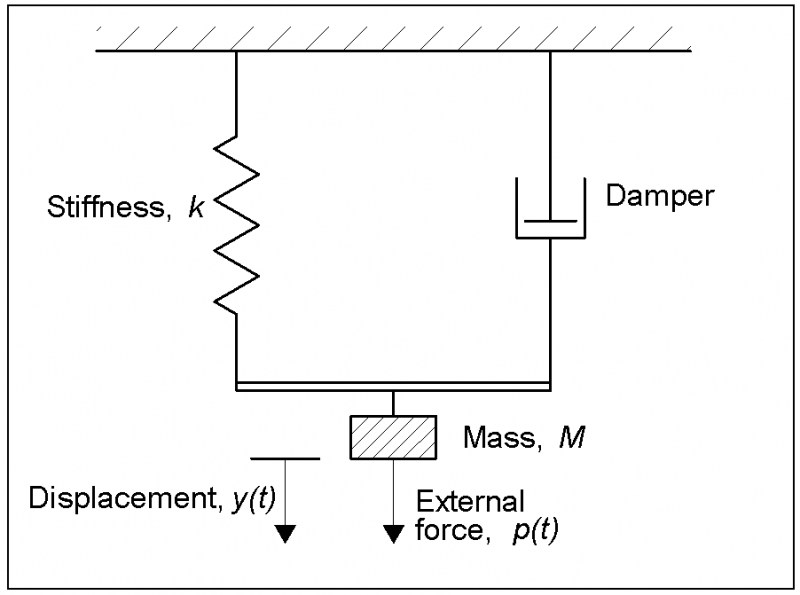
\includegraphics[scale = 0.4]{figures/single_degree.png}  
\end{figure}

\section{Time Series}
\paragraph{}
A time series is a sequence of the data points on a particular variable. Generally, each data points should be taken at a constant intervals as seconds, minutes, hours, days, months, and years.  The different procedure of time series is that the lag values of the target variable are used to predict the value of the target variable as predictor variable. On the other hand, the traditional other types of model do not require target variable as predictors since the historical data has no dependence to current or future data. 

\paragraph{}
There are many diverse techniques in order to analyze sequential data. However, the original technique started from a special case of regression analysis \cite{dash_2020} which is different from normal regression. Time series consist of four different elements as following:
\begin{itemize}
\item Seasonal variations: the repeats of shape or appearance occur during a specific period such as daily, weekly, monthly, season, etc.
\item Trend: it contains 3 different type as up trend, down trend, and sideway which can be linear or non-linear.
\end{itemize}
\begin{itemize}
\item Cyclical variations: its movement depends on its cyclic such as business cycles. it has a similar behavior as seasonal variations but has a longer period.
\item Random variations: this situation when the sequential data does not belong to 3 categorize above.
\end{itemize}

\subsection{Autoregressive (AR)}
\paragraph{}
Actually, autoregressive models which use for predict or forecast proposes operate under the condition that the current value depends on the past values. The equation of autoregressive is shown below:

\hfil $Y_t = \varphi_1Y_{t-1} + \cdots + \varphi_pY_{t-p} + \epsilon_t $ \par 

Where  is white noise and  is a parameter coefficient. For example, AR(1) means the current value is based on the immediately value. AR(2) means the current values is based the previous two values.

\subsection{Dynamic Time Warping (DTW)}
\paragraph{}
Since the last two decades, one of the most challenging problems in data mining is a classification in time series \cite{ismail_fawaz_forestier_weber_idoumghar_muller_2019}. There are several methods to solve this task. Specifically, the Dynamic Time Warping (DTW) can be outstanding as a strong baseline, which the current state-of-the-art is non deep classifier. The dynamic time warping which use for classification is a popular technique to provide the best distance and alignment trajectory between two sequential data which can stretch or shrink to accommodate variations in the time axis as well \cite{dynamic_time_warping_2007}. The equation of DTW is shown below, where D(i,j) refer to the dynamic time warping distance between the subsequences: Figure \ref{fig:DTW}

\hfil $ D(i,j) = \| x_i - y_j \|$ + $min$ $\begin{cases} $D(i-1, j  )$ \\ $D(i-1, j-1)$ \\$D(i  , j-1)$ \end{cases}$  \par 

\begin{figure}[H]
  \centering
  \caption[The different of Euclidean and DTW matching.]{\emph{The different of Euclidean and DTW matching. \\
  Reprinted from Dynamic time warping on Wikipedia}}\label{fig:DTW}
  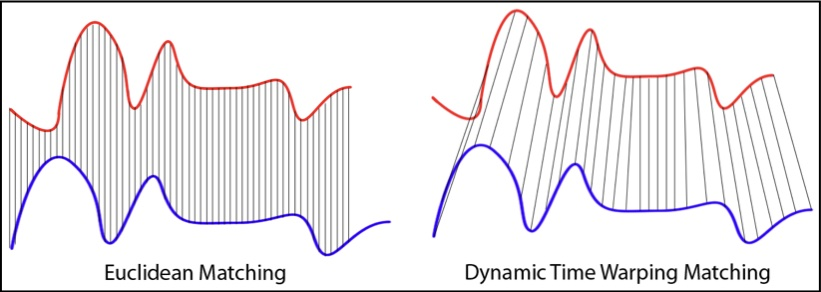
\includegraphics[scale = 0.5]{figures/DTW.jpg}  
\end{figure}

\paragraph{}
In addition, this technique can be used not only for pattern matching or classification, but also anomaly detection when the distance of two signal is higher than set threshold. However, the weaknesses of dynamic time warping are that it consume long processing time, and still lacking complete solutions and development. That why this method is not widely used commercially.

\subsection{Convolution Neural Network (CNN)}
\paragraph{}
A Convolution Neural Network is a deep learning algorithm, which input can be image, spatial or 2 dimension data and also 1 dimension data. This allows CNN to be used in more general data type including texts and other time series data. CNN can be able to successfully capture the spatial and temporal dependencies in the data through the relevant filters as called convolution. A convolution is a sliding a filter though the time series as shown in Figure \ref{fig:CNN} and its general equation is shown in equation below:

\hfil $C_t = f(W \cdot X_{t-l/2 \to t+l/2} + b) | \forall t \in [1, T] $ \par \

\begin{figure}[H]
  \centering
  \caption[Convolving on univariate input time series]{\emph{Convolving on univariate input time series \\
  Reprinted from work of \citeauthor{ismail_fawaz_forestier_weber_idoumghar_muller_2019} \citeyear{ismail_fawaz_forestier_weber_idoumghar_muller_2019}}}\label{fig:CNN}
  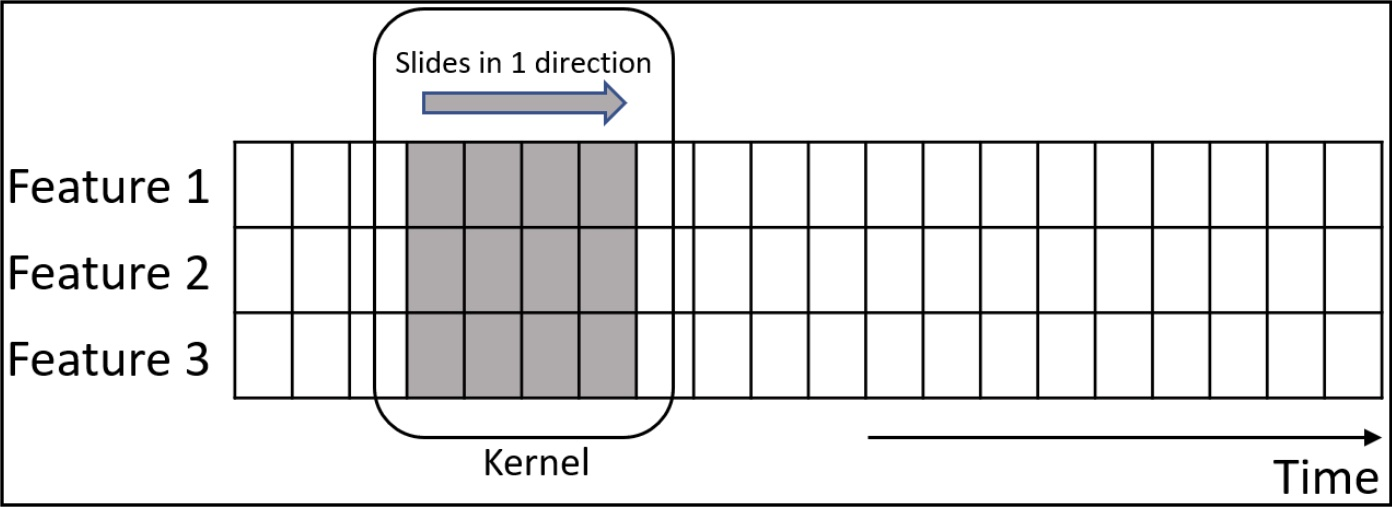
\includegraphics[scale = 0.3]{figures/CNN.jpg}  
\end{figure}


Where $C_t$ is the result of a convolution at time $t$ on a univariate time series $X$ of length $T$ with a filter $W$ of length $l$ , a bias parameter $b$ and a final non-linear function $f$. It can be noticed that the same filter values $W$ and bias $b$ is a very significant useful property called weight sharing. When finishing convolution, those information must be fed though fully-connected layer as same as simple neural network architecture as shown in Figure \ref{fig:CNN_ts}.

\begin{figure}[H]
  \centering
  \caption[Fully Convolutional Neural Network architecture.]{\emph{Fully Convolutional Neural Network architecture.  \\
  Reprinted from work of \citeauthor{ismail_fawaz_forestier_weber_idoumghar_muller_2019} \citeyear{ismail_fawaz_forestier_weber_idoumghar_muller_2019}}}\label{fig:CNN_ts}
  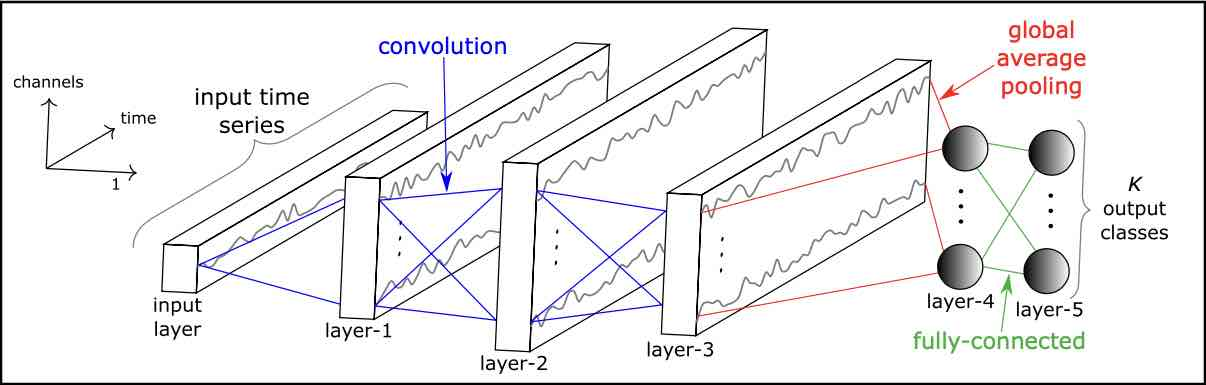
\includegraphics[scale = 0.3]{figures/CNN_ts.jpg}  
\end{figure}



\section{Autoencoder}
\paragraph{}
Basically, an autoencoder is an artificial neural network which can be able to compress data as similar as what it has been trained. The important thing is that to train a model, it does not require labeled data since an autoencoder is an unsupervised model, just feed the raw input into it. As shown in Figure \ref{fig:ae}, this illustrated the intuition of how an autoencoder works. In addition, it can use for denoising form the original data, this is training autoencoder to reproduce the original input from a noisy input. This allow the autoencoder to be flexible with white noise data and capture only useful pattern of the data \cite{vincent10a}.

\begin{figure}[H]
  \centering
  \caption[How does an autocoder work?]{\emph{How does an autocoder work? \\
  Reprinted from work of \citeauthor{chollet_2016} \citeyear{chollet_2016}}}\label{fig:ae}
  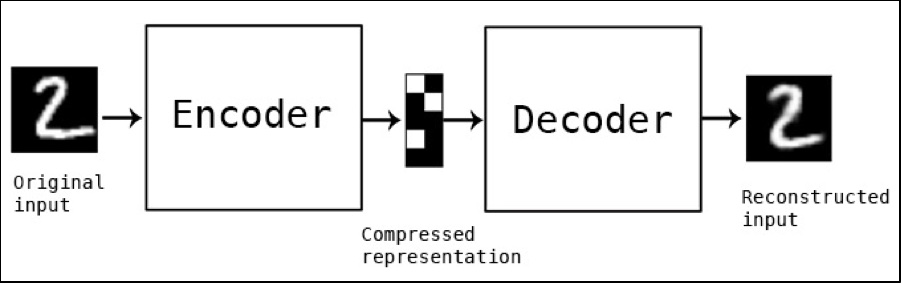
\includegraphics[scale = 0.5]{figures/ae.jpg}  
\end{figure}

\paragraph{}
An autoencoder has 3 main components \cite{badr_2019} as encoder, code or bottleneck and decoder as shown in Figure \ref{fig:ae_architecture}.
\begin{itemize}
\item Encoder: The model learns how to reduce the input dimensions and compress the input data into an encoded representation.
\item Bottleneck: The layer that contains the compressed representation of the input data. This is the lowest possible dimensions of the input data, also called latent space.
\item Decoder: The model learns how to reconstruct the data from the encoded representation to be as close to the original input as possible.
\end{itemize}

\begin{figure}[H]
  \centering
  \caption[The autoencoder architecture.]{\emph{The autoencoder architecture. \\
  Reprinted from work of \citeauthor{pedamkar_2019} \citeyear{pedamkar_2019}}}\label{fig:ae_architecture}
  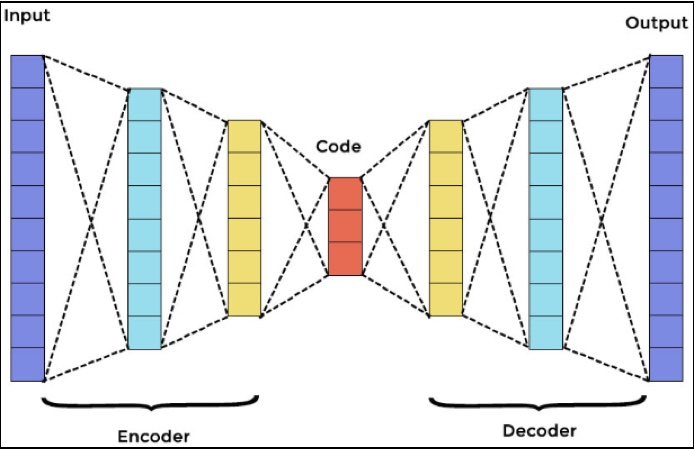
\includegraphics[scale = 0.5]{figures/ae_architecture.jpg}  
\end{figure}

\paragraph{}
The indirect benefits of this model is that it can use for dimensional reduction \cite{rajan_2021}. You can notice that in the bottleneck, the number of neural node is the smallest. Thus, it means the feature of input also be forced to reduces its features. An example of reduced feature by using autoencoder as illustrated in Figure \ref{fig:ae_f_reduction}. It is reduced from 3 to 2 dimensions.


\begin{figure}[H]
  \centering
  \caption[The dimensionality reduction by using autoencoder.]{\emph{The dimensionality reduction by using autoencoder.  
  Reprinted from work of \citeauthor{the_swiss_roll_2015} \citeyear{the_swiss_roll_2015}}}\label{fig:ae_f_reduction}
  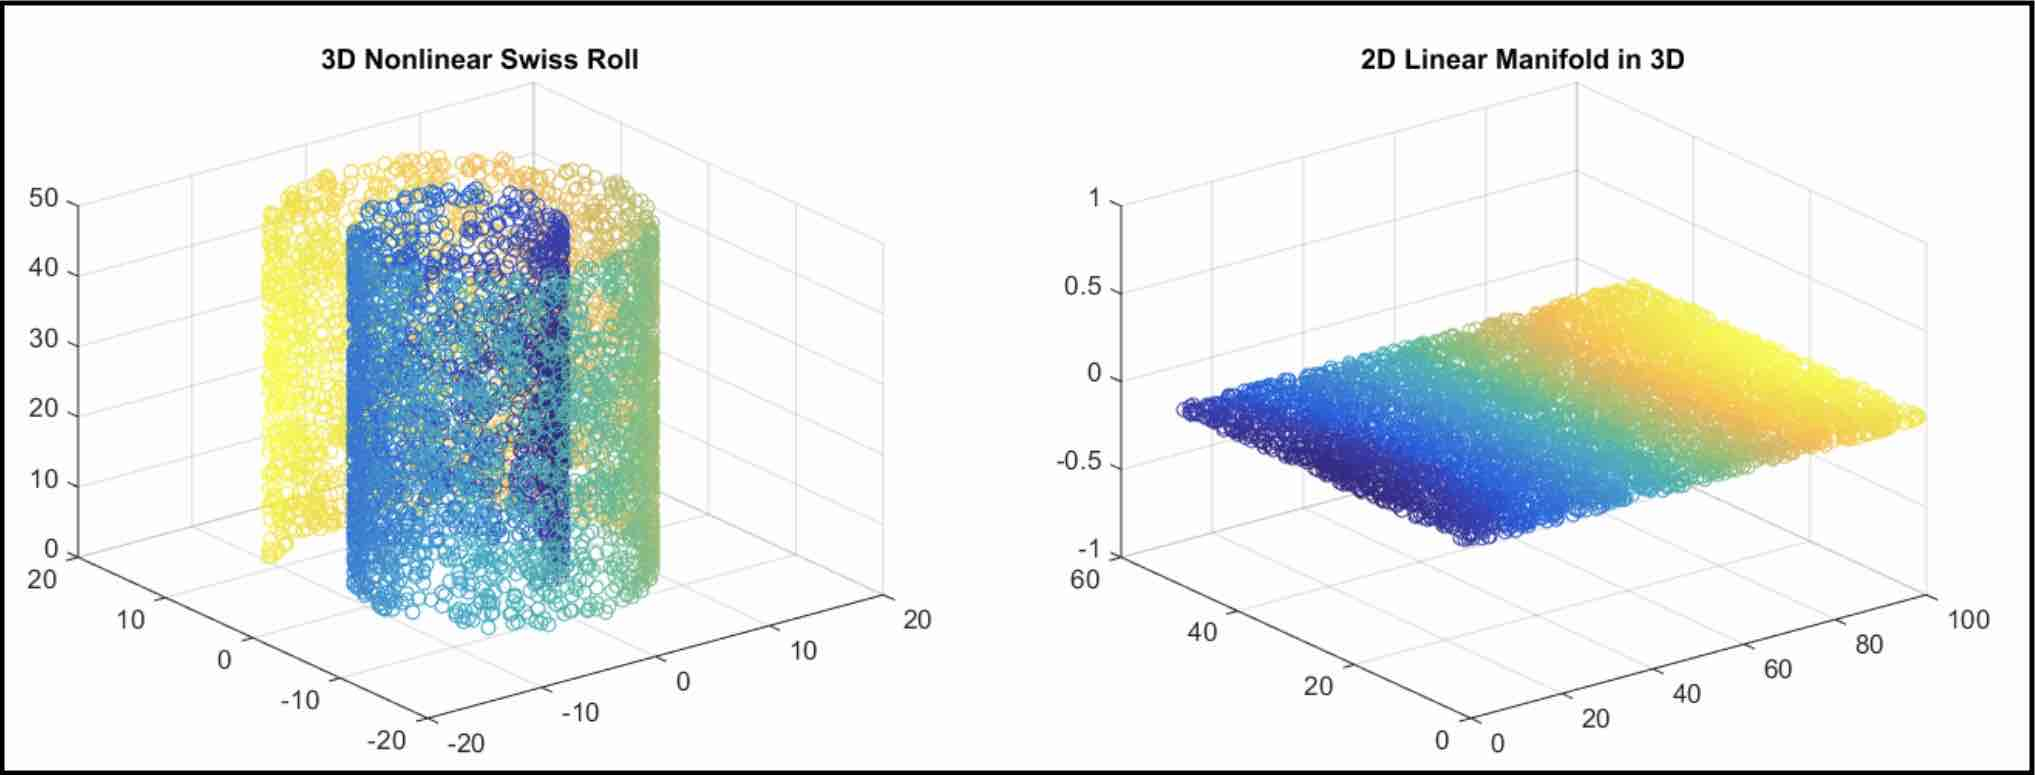
\includegraphics[scale = 0.2]{figures/ae_f_reduction.jpg}  
\end{figure}


\paragraph{}
The other magic of an autoencoder is that when the input is wrong or has some noises, the model is going to correct it as shown in Figure \ref{fig:ae_2}. This is because optimizer is trying to create the output that matches the trained value as much as possible. \citeauthor{vincent_larochelle_bengio_manzagol_2008} \citeyear{vincent_larochelle_bengio_manzagol_2008} found that the robustness of their internal layers (i.e., bottom neck representation) are developed by adding noise to the original input.


\begin{figure}[H]
  \centering
  \caption[An autoencoder tries to correct the output.]{An autoencoder tries to correct the output. \\\hspace{\textwidth}
  \emph{Reprinted from work of \citeauthor{rosebrock_2020} \citeyear{rosebrock_2020}}}\label{fig:ae_2}
  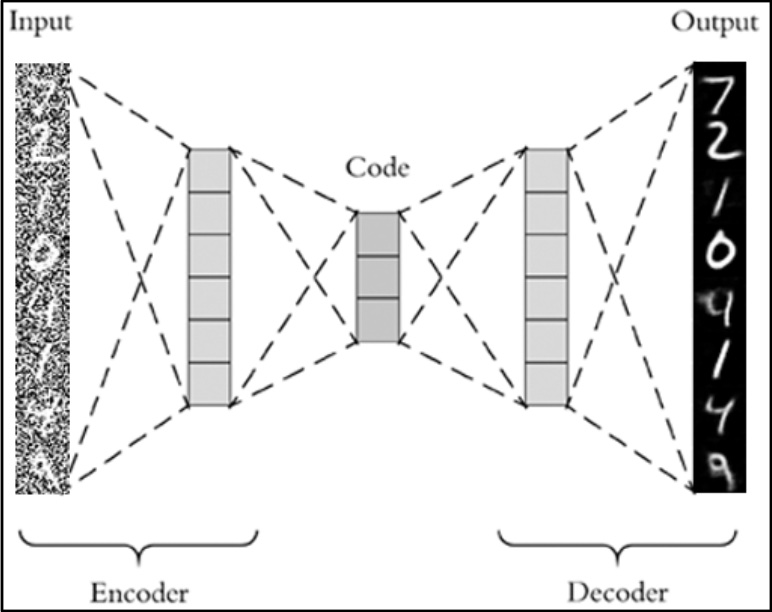
\includegraphics[scale = 0.4]{figures/ae_2.jpg}  
\end{figure}

\paragraph{}
In addition, the network architecture of autoencoders which contain neural network can be adapted between a simple feedforward network, Long Short Term Memory network (LSTM) or Convolutional Neural Network (CNN) depending on the type of input. Based on my thesis, the input, vibration from human activities, is always in sequential time series. Therefore, an applicant autoencoder with LSTM network architecture may be suitable for my proposal.

\subsection{Autoencoder for Anomaly Detection}
\paragraph{}
The magic of autoencoders is simple and very natural. Let’s take a look at our daily life. We do the same things everyday. But one day, we find that an unusual event has happened. We just consider this event absolutely abnormal. The procedure of an autoencoder is exactly the same. An autoencoder does not need any anomaly data at all. It required only normal data to train the model. And when abnormal situations occur, the model can detect that situation as similar to our daily life and be shown in Figure \ref{fig:ae_detection}. It uses the reconstruction error to make decision which data is abnormal. Firstly, we always feed the normal data into the model to train the autoencoder. Secondly, after training is finished, the model can reconstruct very well on the normal data. And it is going to fail when faced abnormal data which model has never seen before. The simple algorithm is shown in Algorithm \ref{al:anomaly_detection_algorithm}.

\begin{figure}[H]
  \centering
  \caption[An autoencoder knows that an anomaly event occurs]{An autoencoder knows that an anomaly event occurs \\\hspace{\textwidth} \emph{Reprinted from work of \citeauthor{pavithrasv_2020} \citeyear{pavithrasv_2020}}}\label{fig:ae_detection}
  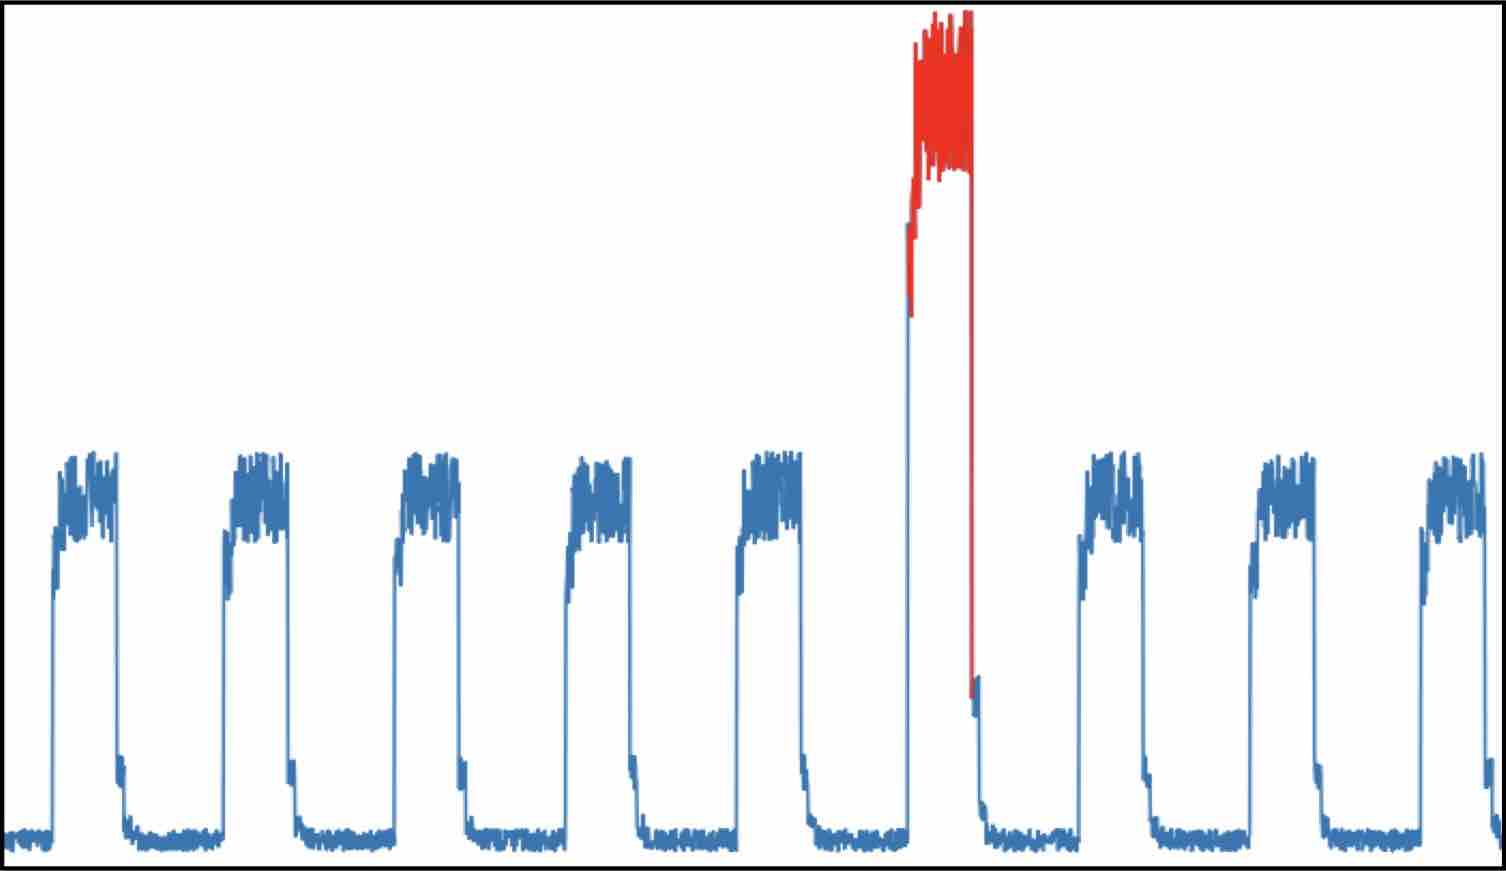
\includegraphics[scale = 0.2]{figures/ae_detection.jpg}  
\end{figure}

\renewcommand{\algorithmicrequire}{\textbf{Input:}}
\renewcommand{\algorithmicensure}{\textbf{Output:}}
\renewcommand{\algorithmicforall}{\textbf{for each}}

\begin{algorithm}[H]
\caption{Autoencoder based anomaly detection }
\label{al:anomaly_detection_algorithm}
\begin{algorithmic}
  \REQUIRE $X$: Normal data
  \ENSURE $\bar{x} $: Reconstruct data
  \STATE $\| X - \bar{x} \|$ : Reconstruction error
  \STATE $\alpha$ : Threshold
  \STATE Step 1 : Train an autoencoder with the normal dataset 
  \STATE Step 2 : Testing the model
  \STATE \indent Step 2.1 : Set a value of $\alpha$
  \STATE \indent Step 2.2 : \textbf{if} reconstruction error $<$ $\alpha$ \textbf{then} $X$ is a normal data
  \STATE \indent \indent \indent \textbf{else} $X$ is an abnormal data
\end{algorithmic}
\end{algorithm}

\subsection{Variational Autoencoder}
\paragraph{}
Basically, Variational Autoencoder (VAE) is a generative model. It estimates the Probability Density Function (PDF) from the training dataset. For example, if model is trained with traffic images, it should provide a high probability value to vehicle images or some object that related with traffic. Otherwise, it should provide a low probability value. In addition, the variational autoencoder can also sample from the learned PDF and generate new examples that look similar to the original dataset \cite{roger_2021}. Or in the other words, a variational autoencoder can be defined as being encoder which is trained to be regularized in order to guarantee that latent space can provide well properties for generative process \cite{rocca_2020}. The architecture of variational autoencoder is illustrated in Figure \ref{fig:VAE}. Thus, the latent space of a variational autoencoder always be sampled from a distribution that encoders learns for each latent feature. 

\begin{figure}[H]
  \centering
  \caption[The architecture of variational autoencoder.]{The architecture of variational autoencoder. \\\hspace{\textwidth} \emph{Reprinted from work of \citeauthor{weng_2018} \citeyear{weng_2018}}}\label{fig:VAE}
  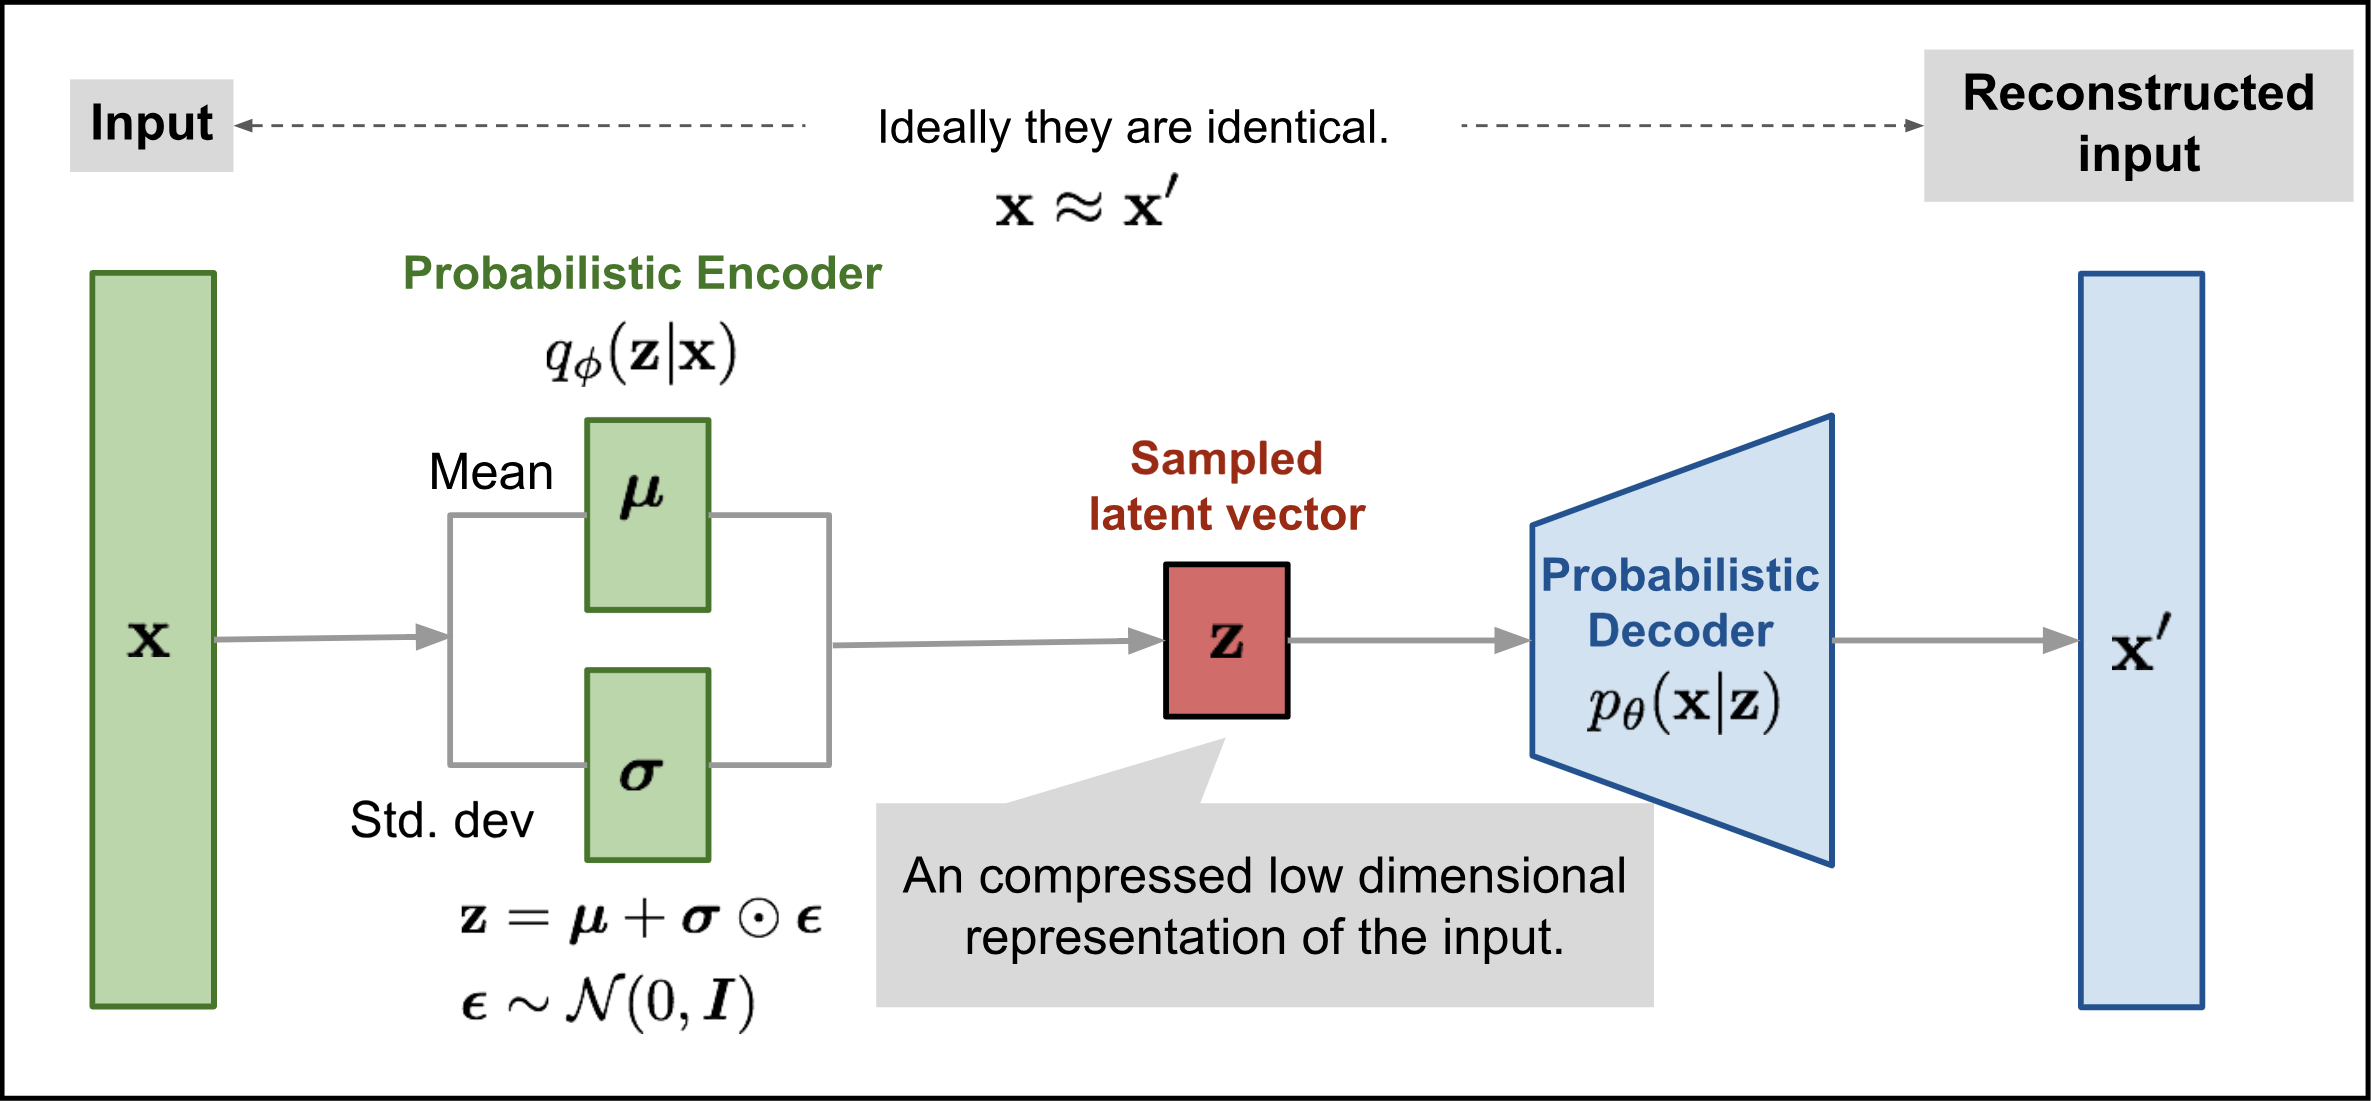
\includegraphics[scale = 0.15]{figures/VAE.jpg}  
\end{figure}

\paragraph{}
Nonetheless, the idea mentioned above does not mean that a variational autoencoder have better performance than general autoencoder in all anomaly detection task \cite{agmon_2021} since the variational autoencoder mostly stands out as a generating new data.


\section{Recurrent Neural Network (RNN)}
\paragraph{}
The main idea of Recurrent Neural Network (RNN) is to apply sequential data such as video (sequence of images) or text (sequence of word). To get more intuition about RNN, for example, when people are reading a book, it is a sequence of words because we read a book from left to right. That we can know what the sentence we are reading is about. We take the story from what we have read in the past (let's call it the hidden state or previous state) and mix it with the words we just read (input data or the words we are reading at that time). RNN uses the same principle, which is to modify the format of the old neural network so that the previous state or knowledge can be added to the new input data to understand something in a sequential time series \cite{donges_2019}. A key attribute of recurrent neural networks is their ability to persist information, or cell state, for use later in the network. There are 2 significant components of RNN as hidden state and input data.


\begin{figure}[H]
  \centering
   \caption[The Recurrent Neural Network architecture.]{The Recurrent Neural Network architecture. \\\hspace{\textwidth} \emph{Reprinted from work of \citeauthor{olah_2015} \citeyear{olah_2015}}}\label{fig:RNN}
  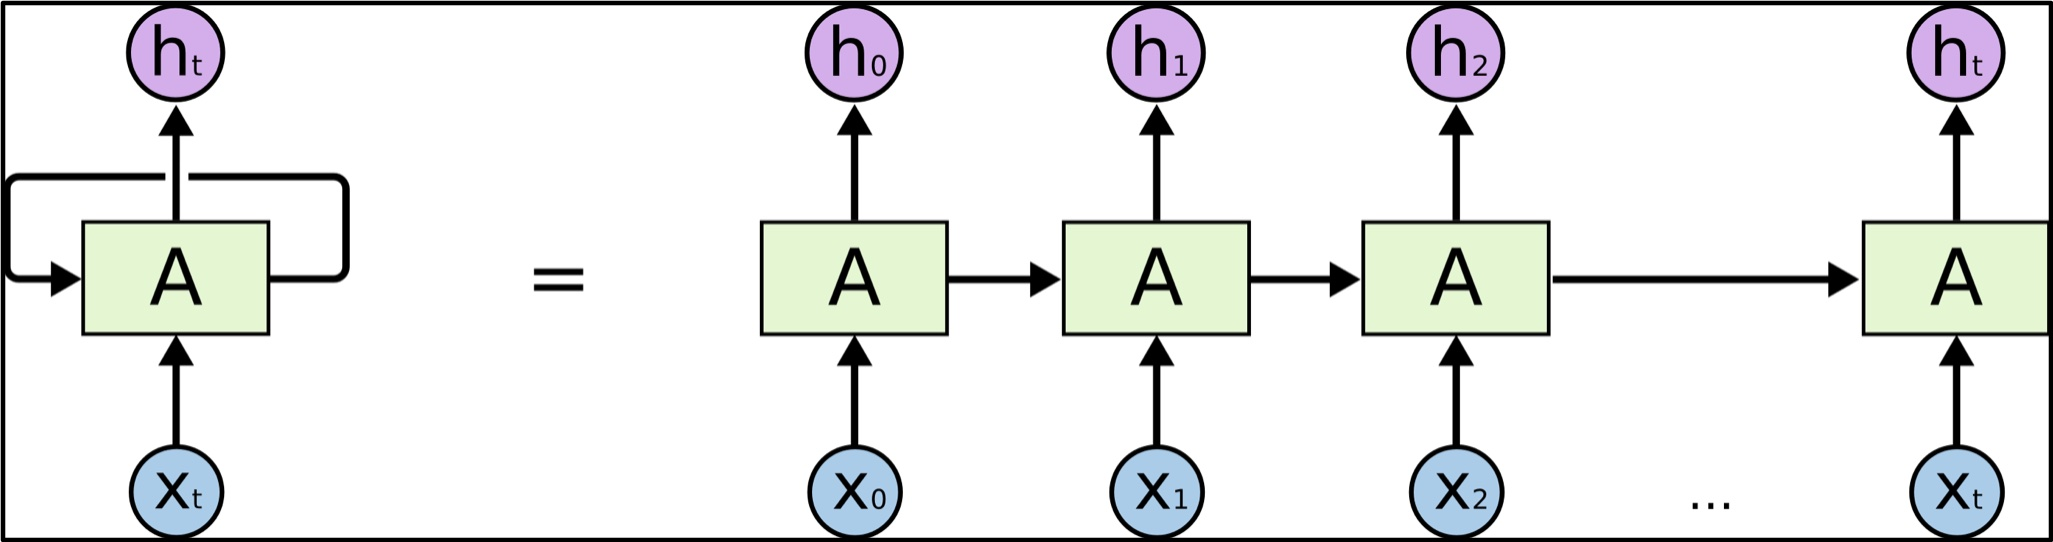
\includegraphics[scale = 0.2]{figures/RNN.jpg}  
\end{figure}

Where $A$ is Hidden layer, $X_t$ is input data at time $t$, and $h_t$ is an output from RNN at time $t$. As shown in Figure \ref{fig:RNN}, on the left shows that there is a loop that loops back into the hidden layer of the Neural Network. As mentioned above, one of the key aspects of the RNN is the previous hidden state and the input data at that time. The main benefit of this loop is to bring back the previous hidden state. (Or we may think of RNN as a Neural Network with more memory to store the previously calculated hidden state). On the right, it is flattened of work step by step.

\paragraph{}
The main problem of RNN is its gradient. For those who have experienced in neural networks would clearly know that to update weights we use a backpropagation algorithm \cite{arnx_2019}, which calculates the gradient of the loss function ($E$) to update the weights which is shown in Figure \ref{fig:bpp}, but RNN is a bit more complicated. Because getting the output $h_t$ is not only from the interval $t=t$, but from $t=t-1, t-2, ....$ all the way to $t=1$ (via Use the hidden state and input data of the previous one, the previous one, the previous one, and so on).

\begin{figure}[H]
  \centering
  \caption[The concept of optimization in a feed-forward neural network.]{The concept of optimization in a feed-forward neural network. \\\hspace{\textwidth} \emph{Reprinted from work of \citeauthor{donges_2019} \citeyear{donges_2019}}}\label{fig:bpp}
  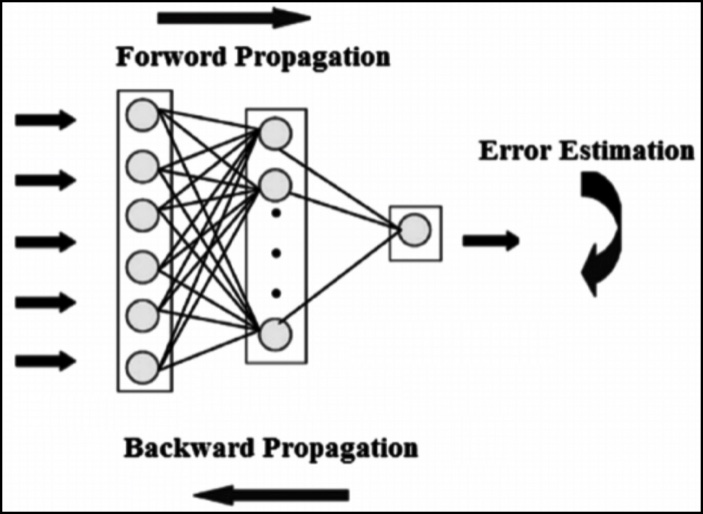
\includegraphics[scale = 0.4]{figures/bpp.jpg}  
\end{figure}

\paragraph{}
Therefore, backpropagation has to be included in all calculations from $t=1$ to $t=t$. Then If the gradient value is less than 1, long continuous multiplications like this will cause the gradient to decrease as the length of its sequence. In explicit, the RNN still has a problem with the data that the sequence is too long.

\begin{figure}[H]
  \centering
  \caption[The repeating module in a standard RNN contains a single layer.]{The repeating module in a standard RNN contains a single layer. \\\hspace{\textwidth} \emph{Reprinted from work of \citeauthor{olah_2015} \citeyear{olah_2015}}}\label{fig:RNN_2}
  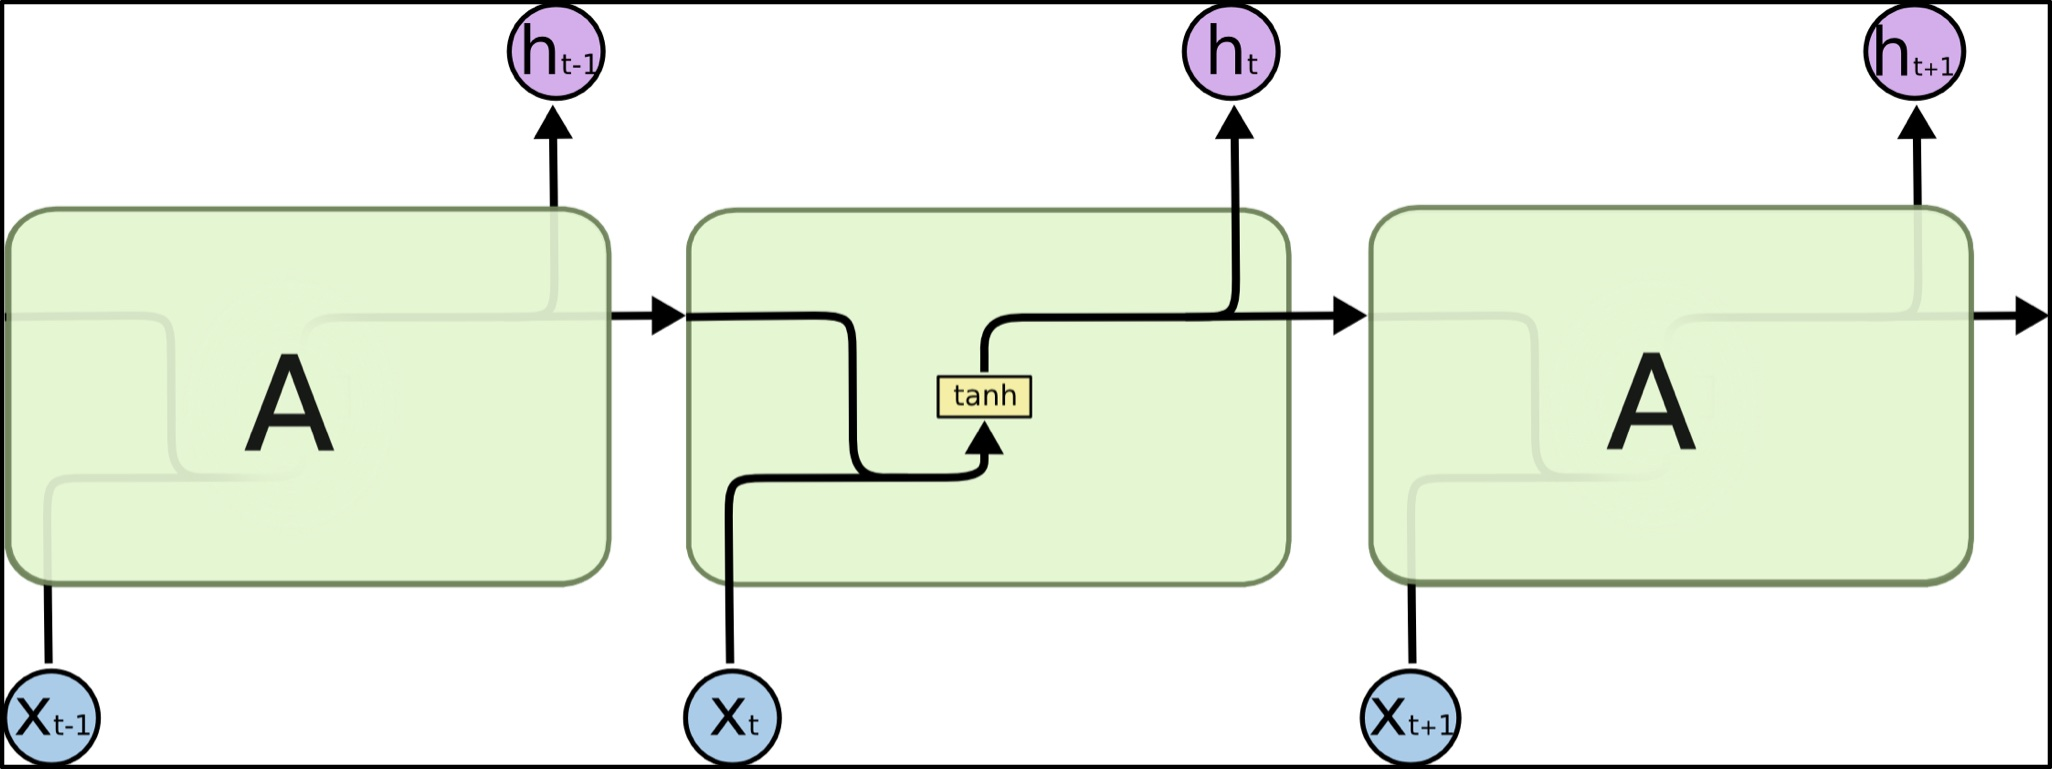
\includegraphics[scale = 0.2]{figures/RNN_2.jpg}  
\end{figure}

\section{Long Short-Term Memory (LSTM)}
\paragraph{}
Long short-term memory networks are an extension for recurrent neural networks, which basically extends the memory. Therefore it is well suited to learn from important experiences that have very long time lags in between \cite{donges_2019,olah_2015}. In addition, memory can also have a descriptor when should write, forget (delete) or read as shown in  Figure \ref{fig:LSTM}.

\begin{figure}[H]
  \centering
  \caption[The procedure inside the LSTM.]{The procedure in the LSTM. \\\hspace{\textwidth} \emph{Reprinted from work of \citeauthor{sirinart_tangruamsub_2017} \citeyear{sirinart_tangruamsub_2017}}}\label{fig:LSTM}
  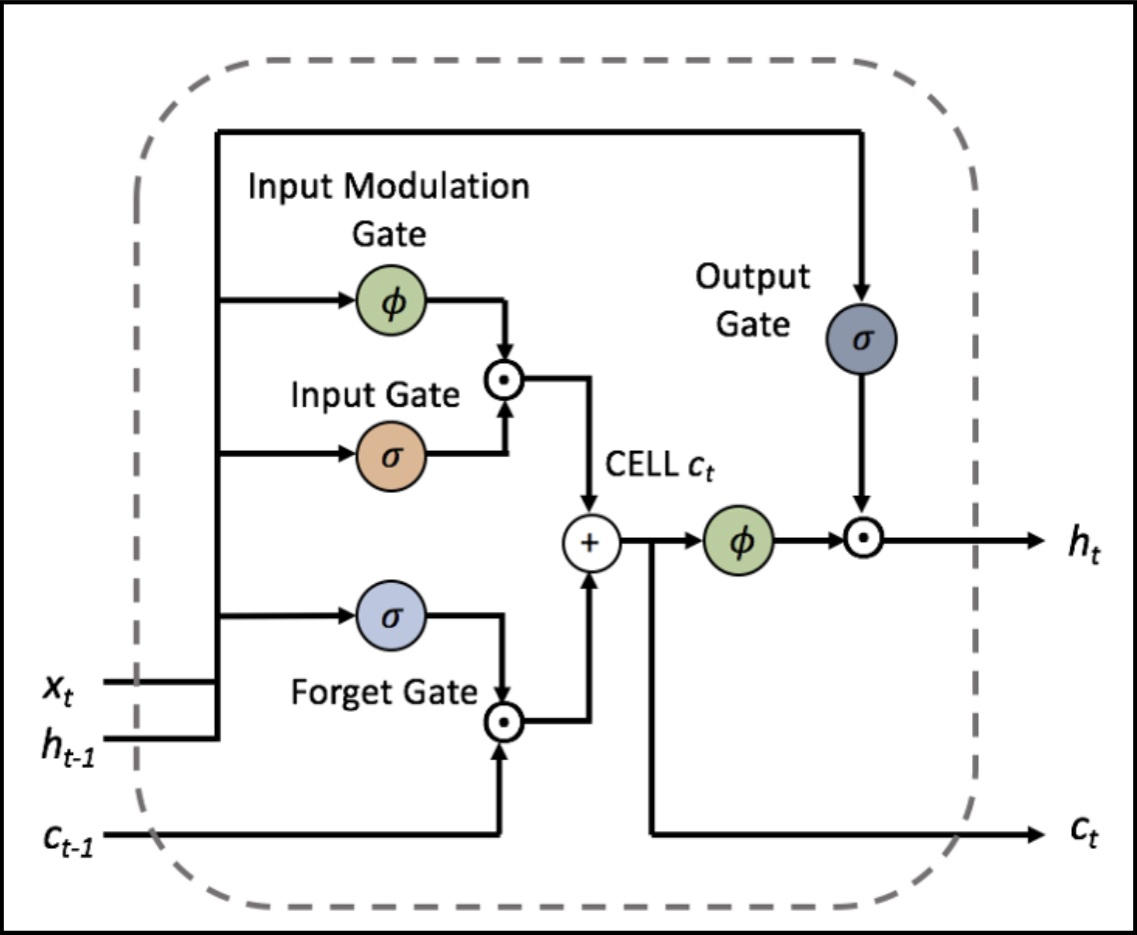
\includegraphics[scale = 0.3]{figures/LSTM.jpg}  
\end{figure}

\paragraph{}
Before getting into the working of LSTM, there are some variables which should be known as following \cite{sirinart_tangruamsub_2017}:
\begin{itemize}
\item Cell state: store the memory state of memory cell the LSTM
\item Gate: control the flow of data, (i.e. analog values) that control when to, write, forget or read. When it should allow data to flow in, flow out or pass away (forget)
\end{itemize}
\paragraph{}
To be more clear, I will explain each functional gate one by one as following :

\paragraph{}
Forget : Forget is like clearing the old cell state (forget it), and preparing to clear memory for the new input. The person who decides whether to delete or not delete is a rule of forget gate. If the forget gate returns 0, then delete the previous cell state. If the forget gate returns 1, the model is going to store this cell state further. To create this forget gate, the model is going to look at the incoming input data with the previous hidden state (according to the RNN formula) for making decisions. The sigmoid function is used as shown in the equation below.

\hfil $ f_t = \sigma(W_{x^f}x_t + W_{h^f}h_{t-1} + b_f) $ \par 

  \paragraph{}
Write : When the new input is fed to the model, it will raise up 2 possible questions as is it good to update cell state with new one and if the model has to update, it will be updated with what value. Firstly, should the model update its cell state? This action is controlled by an input gate which still uses the sigmoid function. This computation which is shown below uses the incoming input data value and the previous hidden state.

\hfil $ i_t = \sigma(W_{x^i}x_t + W_{h^i}h_{t-1} + b_i) $ \par
Secondly, If the model really updates, what value should it update? It is called “Input modulation date” to handle. The equation which is shown below is similar to the input gate, but uses a tanh function instead.

\hfil $ g_t = \tanh(W_{x^c}x_t + W_{h^c}h_{t-1} + b_c) $ \par 

\paragraph{}
Update cell state : Currently, we get information from the forget gate, input gate and input modulation gate which are enough to update cell state. The equation of update cell state will be shown below.

\hfil $c_t = f_t \cdot c_{t-1} + i_t \cdot g_t $ \par 
Let's start with the first part of the equation. You can notice that If the forget gate wants to delete the old cell state ($f_t$ is 0), the model will not let $c_{t -1}$ to update cell state anymore. But if $f_t$ is 1, the model can still keep $c_{t -1}$ to be considered. Let’s come to the latter part of the equation. This section will update the cell state from the new data. Now that model has the values to be updated and waited from the input modulation gate or $g_t$. If $i_t$ is 1, then use $g_t$ to update. Otherwise, $g_t$ is useless.

\paragraph{}
Read : The name here might be confusing. What is it going to read next? Let's skip to explain the output first. From the original RNN, what the model needs to produce is the hidden state at time $t$ or $h_t$. At the time of $t+1$, this LSTM takes this $h_t$ to be calculated. Therefore, the word “read” means to allow outsiders to read the $h_t$ or not. Or it will not pass the $h_t$ value. Here we have an output gate to help the model decide as shown in the equation below. 

\hfil $ o_t = \sigma(W_{x^o}x_t + W_{h^o}h_{t-1} + b_o) $ \par 
And the output will be $h_t$ for the next sequence

\hfil $ h_t = o_t \cdot \tanh(c_t) $ \par 
As you can see, if the output gate provides $o_t$ with 0 value, then ht then is 0 (meaning nothing is sent). Meanwhile, if $o_t$ is 1, the model computes $h_t$ and sends it outside or simply says that it allows others to see the $h_t$ value.

\begin{figure}[H]
  \centering
  \caption[The repeating module in a LSTM contains four interacting layer.]{The repeating module in a LSTM contains four interacting layer. \\\hspace{\textwidth} \emph{Reprinted from work of \citeauthor{sirinart_tangruamsub_2017} \citeyear{sirinart_tangruamsub_2017}}}\label{fig:LSTM_2}
  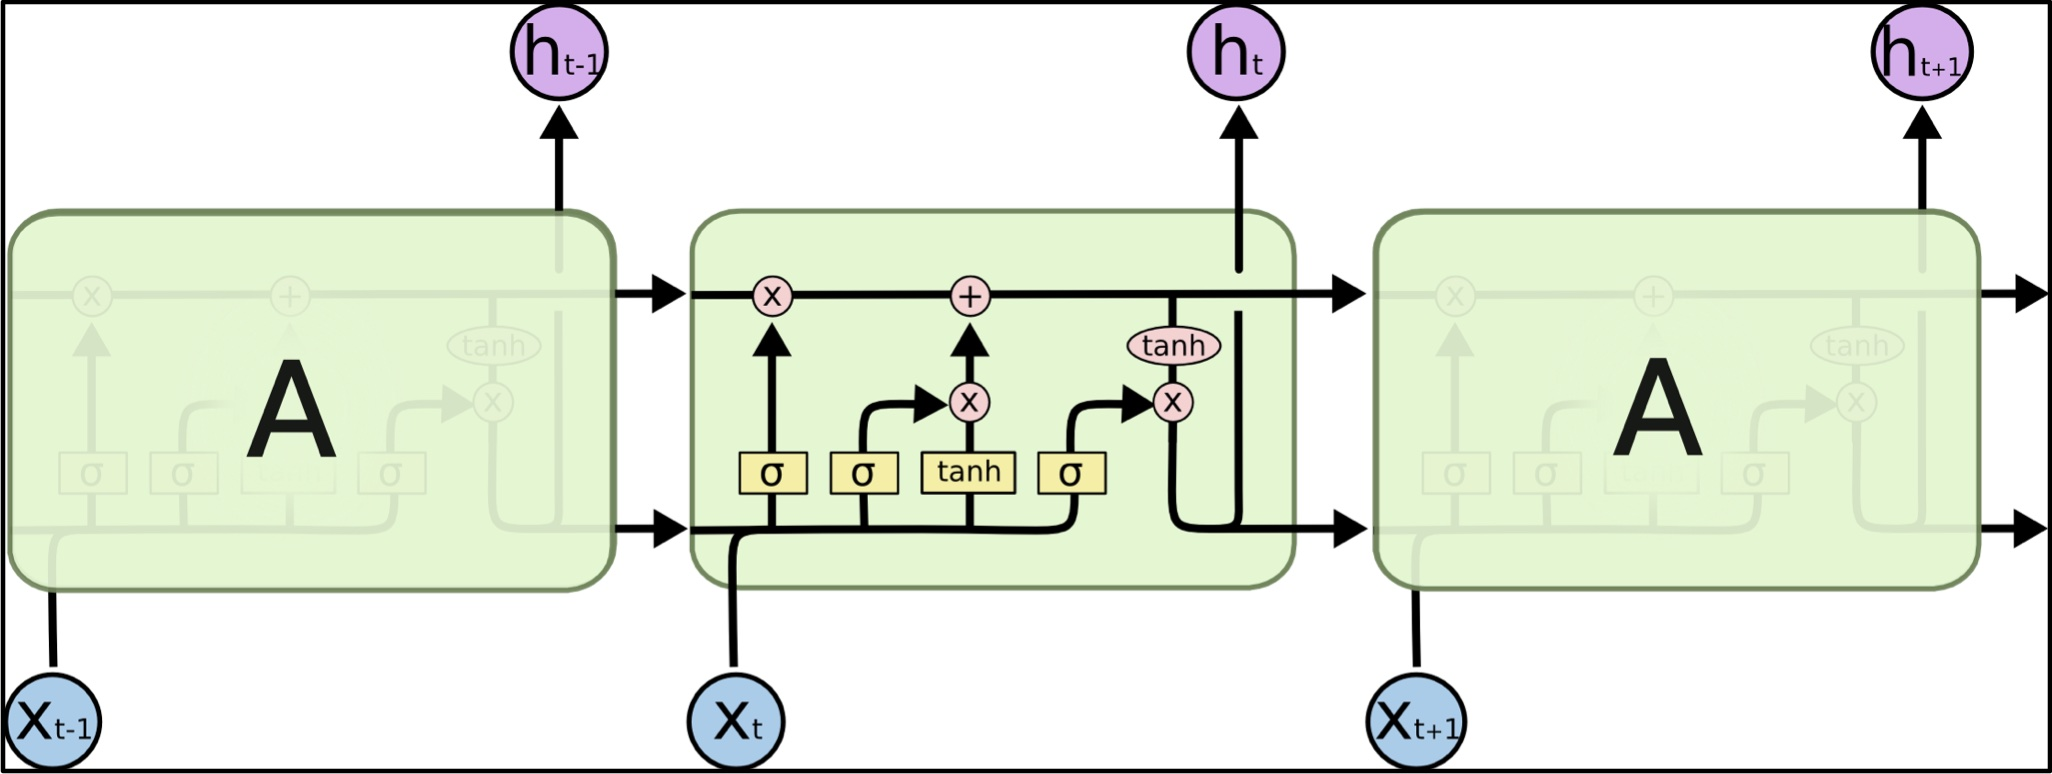
\includegraphics[scale = 0.2]{figures/LSTM_2.jpg}  

\end{figure}

\section{Transformer}
\paragraph{}
The Transformer was proposed in the paper Attention is All You Need by Google \cite{vaswani_shazeer_parmar_uszkoreit_jones_n_gomez_kaiser_polosukhin_2017}. This paper proposes a new architecture that replaces RNNs with attention called Transformer as shown in Figure \ref{fig:attention}. Transformer architecture has continued to beat benchmarks in many domains. Explicitly, it has revolutionized the Natural Language Processing (NLP) field particularly on the machine learning task. This model contains 2 significant parts as an encoder and decoder which can work as similar as an autoencoder. Thus, it can be used for anomaly detection purposes as well.

\begin{figure}[H]
  \centering
  \caption[The Transformer architecture.]{The Transformer architecture. \\\hspace{\textwidth} \emph{Reprinted from work of \citeauthor{vaswani_shazeer_parmar_uszkoreit_jones_n_gomez_kaiser_polosukhin_2017} \citeyear{vaswani_shazeer_parmar_uszkoreit_jones_n_gomez_kaiser_polosukhin_2017}}}\label{fig:attention}
  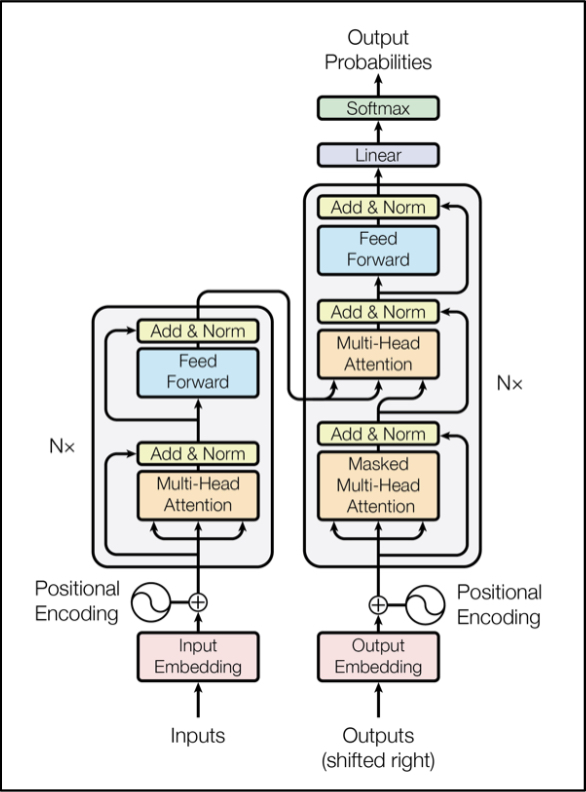
\includegraphics[scale = 0.4
  ]{figures/attention.jpg}  
\end{figure}

\paragraph{}
Let’s compare RNNs and attention, RNNs include every information that they had known about a sequential data into the final hidden state of the network. Thus, the decision layer can access only the memory layer which is related to that time step. It means that at every time step, it focuses on different positions on the other RNN. On the other hand, an attention mechanism regards the input from several time steps and sets different weights to each input to know which input should be focused in order to make one prediction. In Figure \ref{fig:rnnvsattention}, this image is going to provide simple intuition of both methods.

\begin{figure}[H]
  \centering
  \caption[Comparison RNNs and Attention.]{Comparison RNNs and Attention.\\\hspace{\textwidth}}\label{fig:rnnvsattention}
  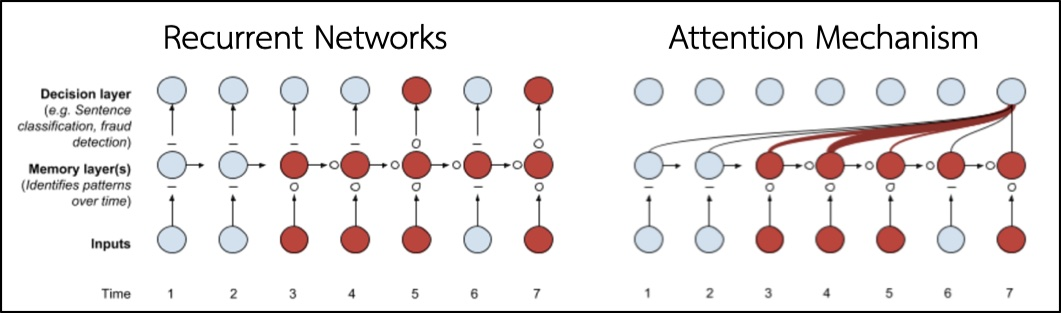
\includegraphics[scale = 0.4
  ]{figures/rnnvsattention.jpg}  
\end{figure}
\subsection{Attention}
\paragraph{}
As you can have a doubt what is the Attention. In psychology, attention is  a concentration of mind on a single object or thought, especially one preferentially selected from a complex, with a view to limiting or clarifying receptivity by narrowing the range of stimuli. Similarly, attention was specifically designed to focus on only the most important subsets of long sequences which are related to completeness of a given task \cite{alammar_2018,alammar_2019,klingenbrunn_2021}. It actually consists 3 main steps as following:
\begin{enumerate}
\item Create the Query, Key, and Value vectors for each path and each input token by multiplying by weight matrices as $W^Q$, $W^K$ and $W^V$ as shown in Figure \ref{fig:attention_2}.
\item For each input token, use its query vector to get a score against all the other key vectors by multiplying the current Query vector with all the Key vectors as shown in Figure \ref{fig:attention_3}.
\item Sum up the Value vectors after multiplying them by their associated scores. The more transparent means lower value as shown in Figure \ref{fig:attention_4}.
\end{enumerate}

\paragraph{}
Therefore, If the model does the same operation for each input token, it is going to finish with a vector which represents the appropriate context of each token as shown in Figure \ref{fig:attention_5}. And these vectors are going to the next sub layer in the transformer block which must be fed into the forward neural network.
\begin{figure}[H]
  \centering
  \caption[Create the query, key and value vector.]{Create the query, key and value vector. \\\hspace{\textwidth} \emph{Reprinted from work of \citeauthor{alammar_2018} \citeyear{alammar_2018}}}\label{fig:attention_2}
  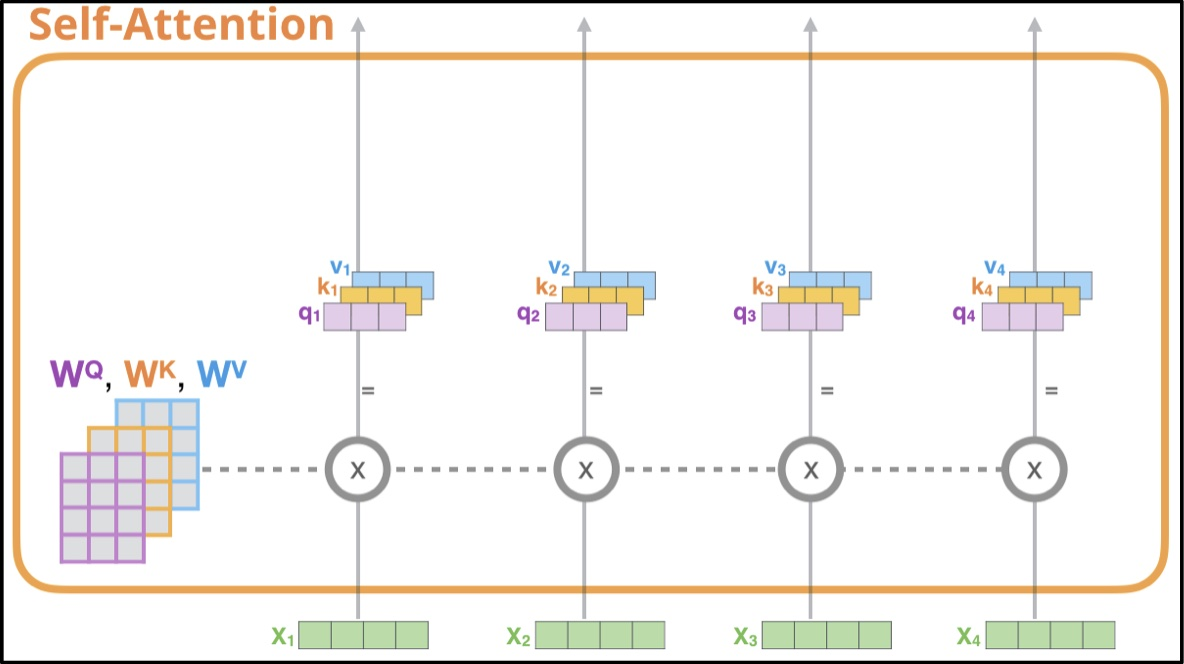
\includegraphics[scale = 0.3]{figures/attention_2.jpg}  
\end{figure}

\begin{figure}[H]
  \centering
  \caption[Get score of how they match.]{Get score of how they match. \\\hspace{\textwidth} \emph{Reprinted from work of \citeauthor{alammar_2018} \citeyear{alammar_2018}}}\label{fig:attention_3}
  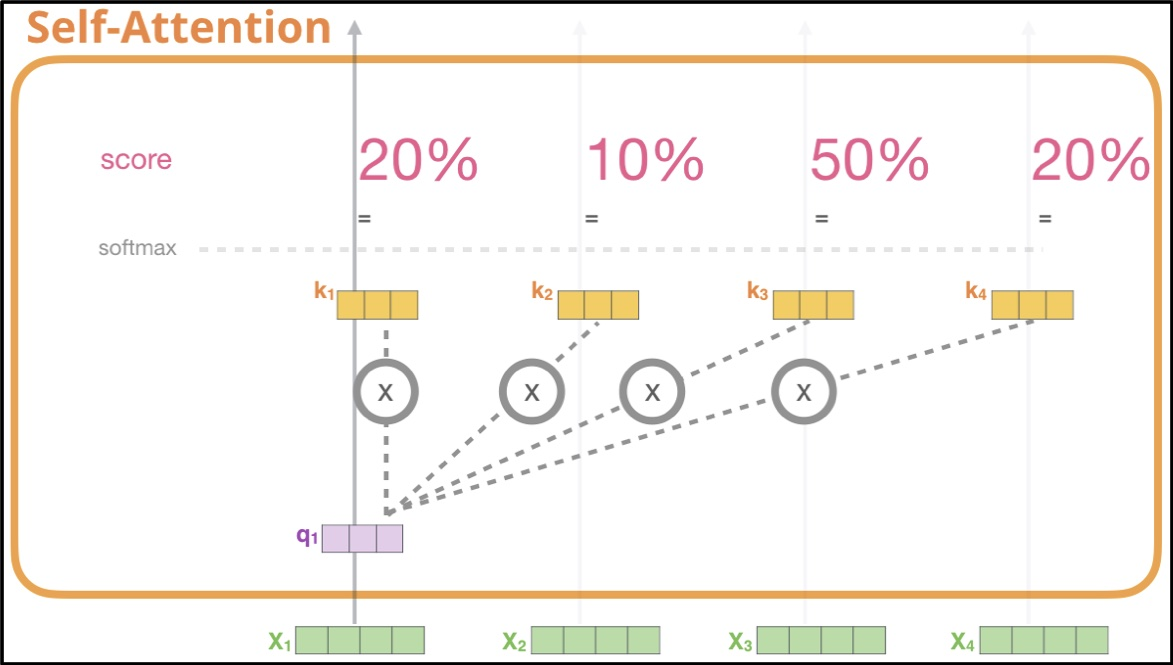
\includegraphics[scale = 0.3]{figures/attention_3.jpg}  
\end{figure}

\begin{figure}[H]
  \centering
  \caption[Sum up the value vectors.]{Sum up the value vectors. \\\hspace{\textwidth} \emph{Reprinted from work of \citeauthor{alammar_2018} \citeyear{alammar_2018}}}\label{fig:attention_4}
  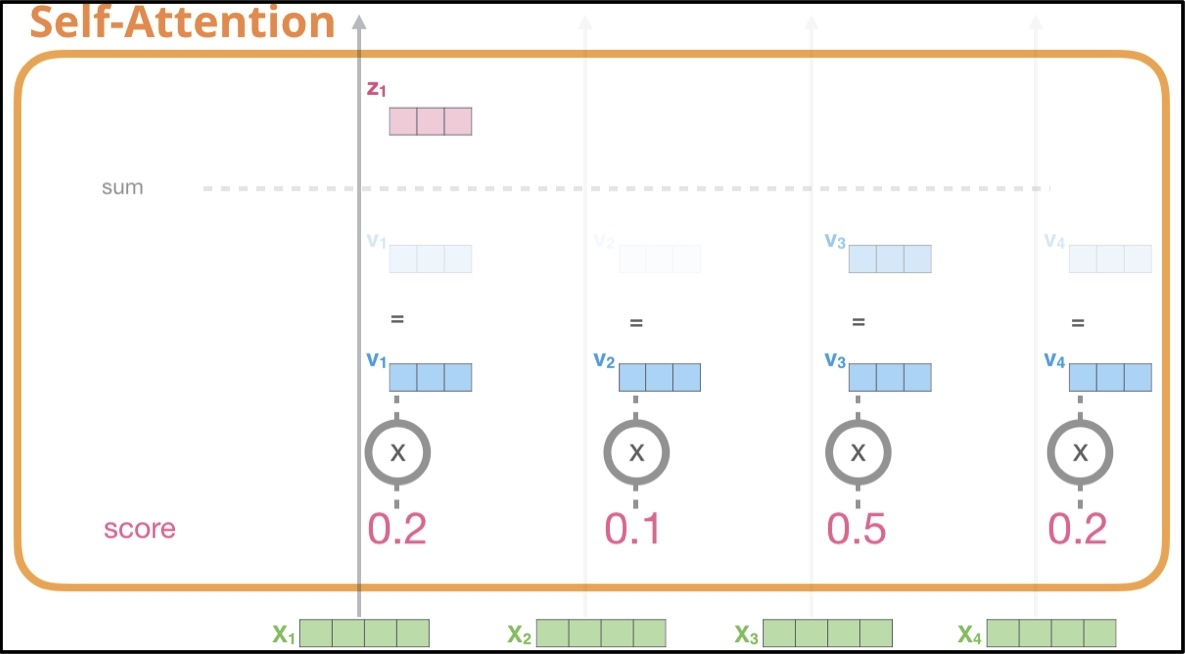
\includegraphics[scale = 0.3]{figures/attention_4.jpg}  
\end{figure}
\begin{figure}[H]
  \centering
  \caption[The outcome after finishing the Attention process.]{The outcome after finishing the Attention process. \\\hspace{\textwidth} \emph{Reprinted from work of \citeauthor{alammar_2018} \citeyear{alammar_2018}}}\label{fig:attention_5}
  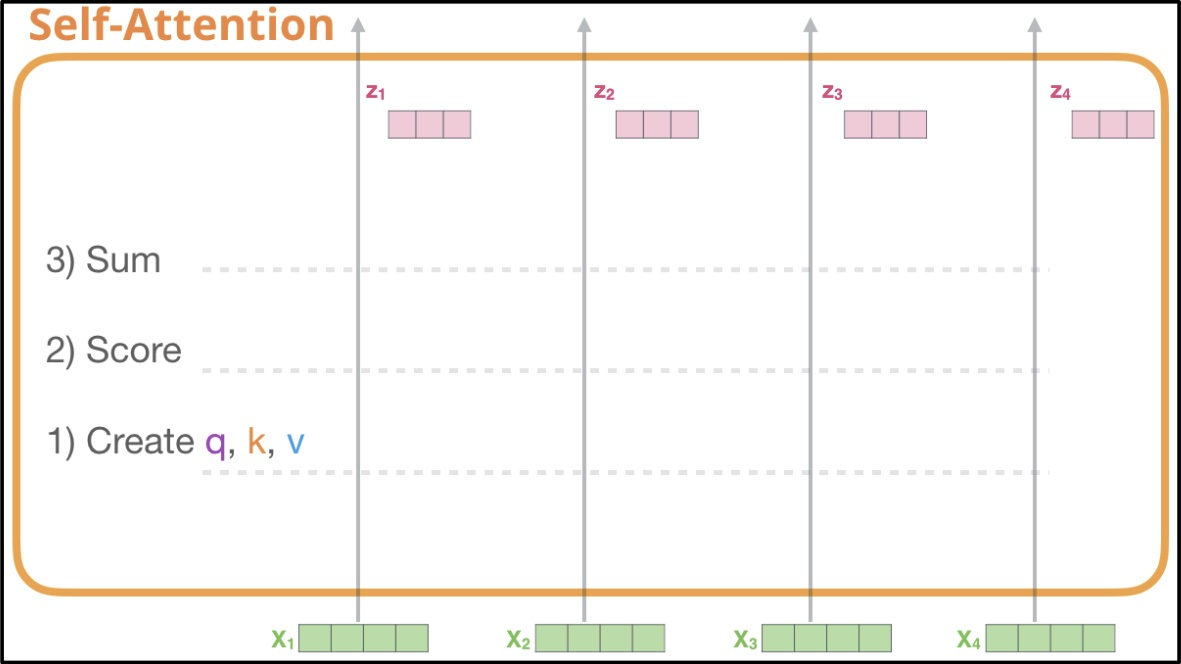
\includegraphics[scale = 0.3]{figures/attention_5.jpg}  
\end{figure}

\paragraph{}
In addition, it can be noticed that in the decoder, it contains Masked Self-Attention. It is very important that the difference between Self-Attention and Masked Self-Attention is quite clear when you look at Figure \ref{fig:attention_6}. A Self-Attention allows each position to attend to all positions from input but Masked Self-Attention only considers the previous position and including that position in order to preserve the auto-regressive property.

\begin{figure}[H]
  \centering
  \caption[The difference of Self-Attention and Masked Self-Attention.]{The difference of Self-Attention and Masked Self-Attention. \\\hspace{\textwidth} \emph{Reprinted from work of \citeauthor{alammar_2019} \citeyear{alammar_2019}}}\label{fig:attention_6}
  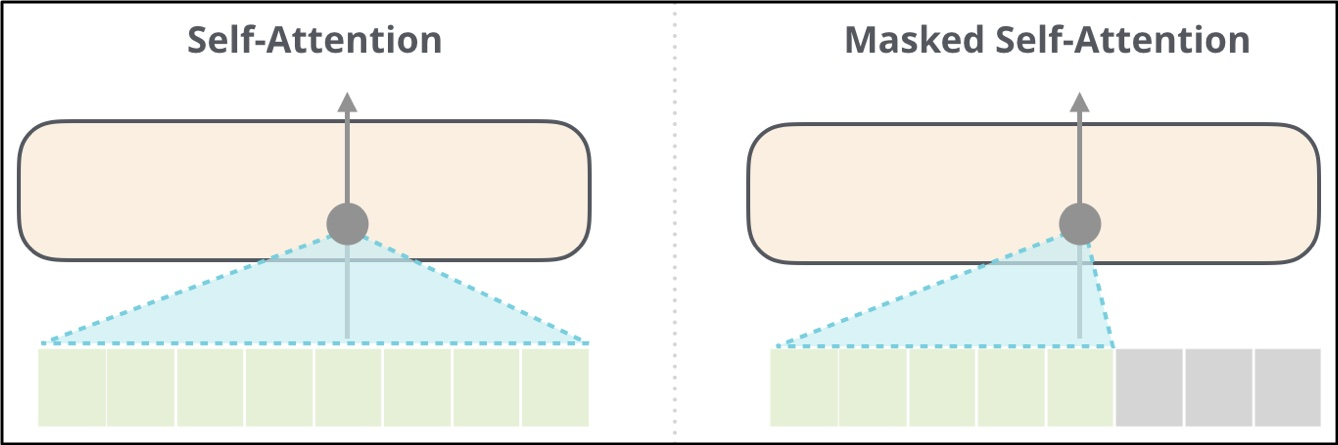
\includegraphics[scale = 0.3]{figures/attention_6.jpg}  
\end{figure}
\subsection{Positional Encoding}
\paragraph{}
For sequence to sequence model, orders and position are important. Since the model does not have recurrence and convolution, we have to add some information to make use of the order in the sequence. You can see in Figure \ref{fig:attention_7}.

\begin{figure}[H]
  \centering
  \caption[The dimension of each positional encoding and embeddings.]{The dimension of each positional encoding and embeddings. \\\hspace{\textwidth} \emph{Reprinted from work of \citeauthor{alammar_2018} \citeyear{alammar_2018}}}\label{fig:attention_7}
  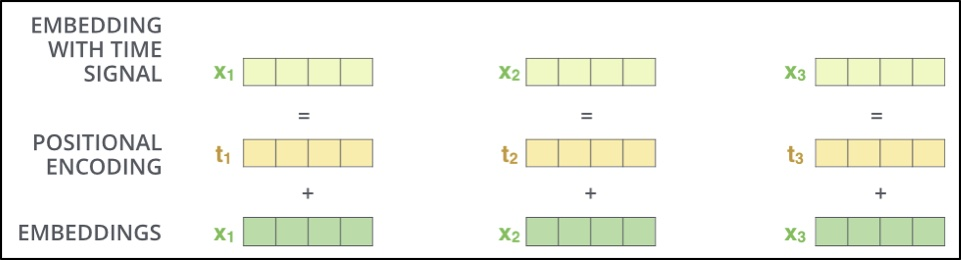
\includegraphics[scale = 0.4]{figures/attention_7.jpg}  
\end{figure}














\FloatBarrier